\documentclass[10pt]{article}
\usepackage[margin=1in]{geometry}
\usepackage{indentfirst}
\usepackage{adjustbox}
\usepackage{listings}
\usepackage{color}
\usepackage{graphics}
\usepackage{hyperref}
\definecolor{dkgreen}{rgb}{0,0.6,0}
\definecolor{gray}{rgb}{0.5,0.5,0.5}
\definecolor{mauve}{rgb}{0.58,0,0.82}
\lstset{frame=tb,
	aboveskip=3mm,
	belowskip=3mm,
	showstringspaces=false,
	basicstyle={\small\ttfamily},
	numbers=none,
	numberstyle=\tiny\color{gray},
	keywordstyle=\color{blue},
	commentstyle=\color{dkgreen},
	stringstyle=\color{mauve},
	breaklines=true,
	breakatwhitespace=true,
	tabsize=3
}
\title{736Paper}
\author{Keith Funkhouser, Malcolm Reid, Colin Samplawski}
\date{Fall 2016}

\begin{document}
\setlength{\baselineskip}{18pt}
\maketitle

\section{Introduction}
Many commonly used C library functions return some value. In most cases, these values indicate something that is relevant to the  functions operations, such as a file descriptor, number of bytes processed, or a pointer to some data. Additionally, many functions that can fail return some predefined value that indicates that an error occurred during the function's execution. Unfortunately, many programmers have the bad habit of not checking these return values for such error conditions, which can lead to unexpected behaviors. In our work, we implemented a mechanism to intercept system/library calls in order to force an error value to be returned to an application. By analyzing how common Linux applications respond (or didn't) to these errors, we were able to evaluate the robustness of these applications.

We were primarily interested in finding crashes in the applications that we tested. By a crash we mean either an unintentional core dump or a hang that could only be ended by forcing the application to terminate (using by a Ctrl-C command). This is a somewhat narrower definition than what is commonly used, but it allowed us to quantify crashes in an unambiguous way. Furthermore, these two cases represent situations where an application terminated without its consent. We require the core dump to be unintentional because core dumps can occur within a programs control, such as with \texttt{abort} or \texttt{assert}. These are somewhat inelegant ways of handling errors, but it does not represent a crash as we define it. Similarly, nearly all of the applications we tested displayed aberrant output that is likely not the behavior the developers intended, but this is simply our opinion and is not something that can be meaningfully measured. Nevertheless, we do include some of the more interesting non-crash behaviors that we found. ROADMAP

It is most interesting to test for unchecked return values in both Unix utilities and large scale programs. We restricted our tests to open-source projects, so we could attempt to find the source code lines that caused the bug. We group the applications that we test into three categories: GNU core utilities, networking utilities, and large open-source projects.

\section{Related Work and Motivation}
Our work is an extension of previous work in fuzz testing. Fuzz testing is conducted by passing randomly generated input to applications in order to find bugs. It was first developed by Miller et al. [?] in 1991. They used it to test how reliable UNIX applications were by counting the number that crashed or hung when passed fuzzed input. Surprisingly, they found that 25-33\% of the applications in the UNIX versions tested crashed or hung. In the same spirit, Miller et al. \cite{bart} fuzz tested more applications in 1995. They found that, although the programs that were tested in the previous study improved in reliability, many programs still crashed or hung. This study also applied fuzzing to test for failure to properly handle error return codes. To test the \texttt{malloc} family of calls, the authors intercepted \texttt{calloc}, \texttt{malloc}, and \texttt{realloc} calls from Unix applications, and with some probability $p$, returned an error value. With probability $1-p$, their program returned the true return code. Of the 53 applications tested, 25 crashed.  We extend this work by increasing both the number of calls and the number of applications tested.  

%As described by the Free Software Foundation, “the GNU core utilities are the basic file, shell and text manipulation utilities of the GNU operating system.” [?]. We selected a representative set of utilities listed in [?]. Net-tools is a set of UNIX applications for viewing and configuring network settings [?]. They have in large part been made obsolete by the “ip” utility. We tested both the Net-tools suite and the “ip” application for unchecked return values. Finally, we decided to test large projects to investigate their reliability. 


\section{Mechanisms}
The main mechanism that we needed was a way of intercepting system and library calls that an application makes in order to control the value returned. We needed a method that would be invisible and non-disruptive to the application being tested. Furthermore, it needed to be fine grained enough so that only calls from the  application being tested would be intercepted.

\subsection{LD\_PRELOAD}
We intercepted system and library calls via the \texttt{LD\_PREOLAD} environment variable. Using \texttt{LD\_PREOLAD} a user can specify a shared library object that is loaded before any others at dynamic linking time. Importantly, functions within this shared library take precedence over any other functions of the same name, even ones found in \texttt{libc} and other standard libraries. For each call we wanted to test, we created a shared library object that contained a single wrapper function with the name of the call of interest. This wrapper would return an error value with probability $p$ or call the real version of the function to allow the application to continue as usual. A visual representation of this mechanism is given in Figure 1.

We used a probabilistic approach in order to test all the calls to a given function within an application. If the error values were returned deterministically, then only the first call to the function would be intercepted. The probability of an error being rets described by the Free Software Foundation, “the GNU core utilities are the basic file, shell and text manipulation utilities of the GNU operating system.” [?]urned had to adjusted depending on the application and the call under testing. Some calls (especially ones related to resource allocation) were called many times within an application, requiring a lower probability, while others were called only a handful of times, requiring a higher probability. We used values from as low as 5\% to as high as 50\%.

\begin{figure}
	\caption{ld\_preload fig}
	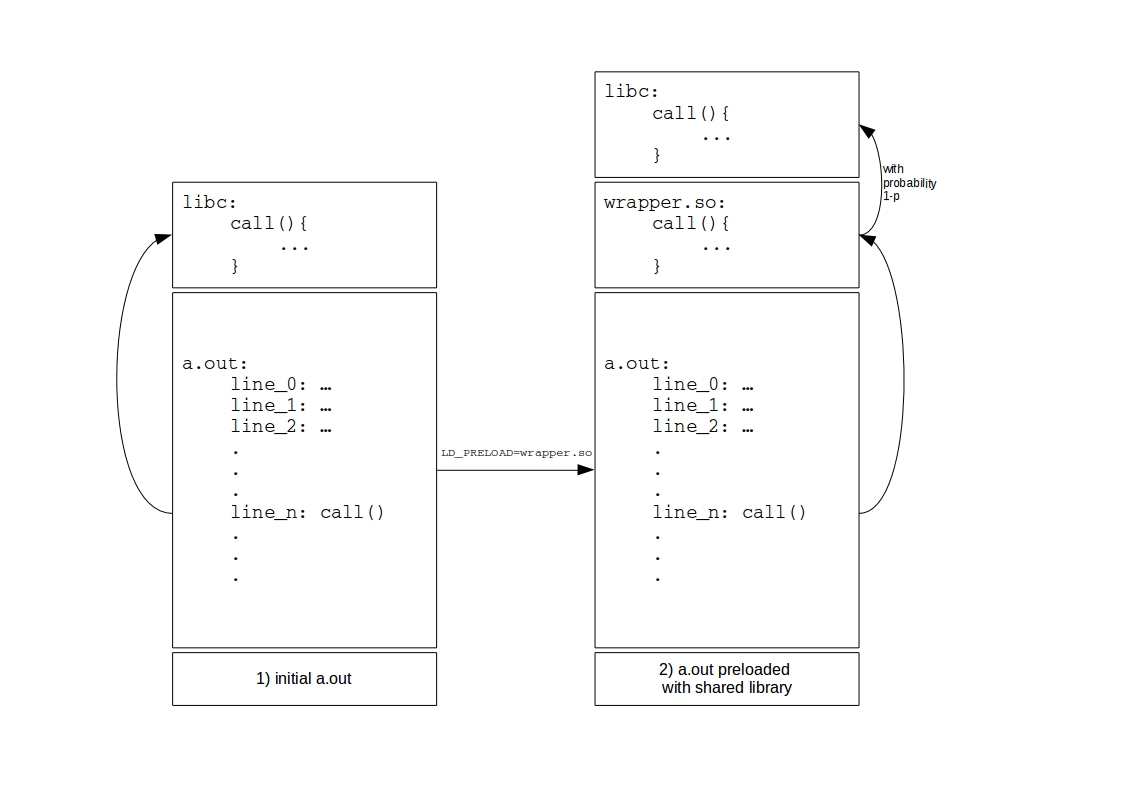
\includegraphics[width=\textwidth]{ldpreload_fig.jpg}
\end{figure}

Calling the original function from within the wrapper is slightly trickier than one might expect. We couldn't simply call the function normally from the wrapper since it would lead to infinite recursion. To break this recursion, we used the \texttt{dlsym} function. \texttt{Dlsym} scans through dynamically loaded libraries looking for the function handle (that is, the address) of a function named as an argument. We can then use the function handle that is returned in order to call the original version of the function. An example of such a wrapper is given in code listing 1.

\begin{minipage}{\linewidth} %minipage so the code is split between two pages
	\lstinputlisting[caption=\texttt{open} wrapper, language=C]{sample_wrapper.c}
\end{minipage}

\subsubsection{Limitations of LD\_PRELOAD}
We chose \texttt{LD\_PRELOAD} primarily because of its simplicity, which allowed us to test a greater number of calls. However there are several limitations to this method. Most significantly, applications that use statically linked libraries bypass our wrappers completely. Fortunately, we never encountered any applications that used static linking. If we wanted to expand coverage to programs that did use static linking we would need to use a binary rewriting tool as used by Miller et al in [?] or a dynamic instrumentation tool such as DynInst [?].

Another limitation to our method is that it is Linux specific. \texttt{LD\_PRELOAD} is found on many Linux distributions and some other UNIX systems, such as BSD \cite{bsd}. There are equivalents found on other popular systems such as the \texttt{AppInit\_DLLs} registry value on Windows \cite{dll} and the \texttt{DYLD\_INSERT\_LIBRARIES} environment variable on macOS \cite{macos}. We feel confident that our method could be applied to applications on these systems, but our current implementation is not portable.

\section{coreutils}

\section{Large scale Programs}

\section{Anecdotes}

\section{Related Work}

\section{Conclusion}

\section{Crashes}
\begin{itemize}

\item \texttt{du/malloc}
\begin{itemize}
\item Return value from \texttt{setup\_dir} is not checked, which allocates memory and returns \texttt{false} in many scenarios, including if \texttt{malloc} fails
\item \url{https://github.com/coreutils/gnulib/blob/master/lib/fts.c#L986}
\item e.g. \texttt{PROB = 0.3}, \texttt{SEED = 10178}
\item Fix:
\begin{lstlisting}
-	setup_dir(sp);

+	if (!setup_dir(sp)) {
+		return NULL;
+	}
\end{lstlisting}
\end{itemize}

\item \texttt{hostid/malloc}
\begin{itemize}
\item In our version of \texttt{libc}, the return value from \texttt{malloc} is not checked, but a counter is set assuming that the return value was valid. This later causes a null pointer dereference.
\item \url{https://github.com/lattera/glibc/blob/master/resolv/res_send.c#L453}
\item e.g. \texttt{PROB = 0.3}, \texttt{SEED = 11589}
\item Fix:
\begin{lstlisting}
	for (ns = 0; ns < statp->nscount; ns++) {
			...
			
	        if (EXT(statp).nsaddrs[ns] == NULL)
	                EXT(statp).nsaddrs[ns] =
	                    malloc(sizeof (struct sockaddr_in6));
+	                if(EXT(statp).nsaddrs[ns] != NULL) {
+	                	EXT(statp).nscount++;
+	                }
			...
	}
-	EXT(statp).nscount = statp->nscount;
\end{lstlisting}
\end{itemize}

\item \texttt{netstat/malloc}
\begin{itemize}
\item Return value from \texttt{malloc} not checked and then passed to \texttt{strcpy}
\url{https://github.com/giftnuss/net-tools/blob/master/lib/inet.c#L213}
\item e.g. \texttt{PROB = 0.3}, \texttt{SEED = 26886}
\item Fix:
\begin{lstlisting}
    pn = (struct add	r *) malloc(sizeof(struct addr));
+   if (pn == NULL) {
+   	perror("netstat");
+		return (-1);
+   }
    pn->addr = *sin;
    pn->next = INET_nn;
    pn->host = host;
    pn->name = (char *) malloc(strlen(name) + 1);
+   if (pn->name == NULL) {
+   	perror("netstat");
+		return (-1);
+   }
    strcpy(pn->name, name);

\end{lstlisting}
\end{itemize}

\end{itemize}


\section*{Appendix}

\begin{thebibliography}{9}
	\bibitem{coreutils}
	http://www.gnu.org/software/coreutils/coreutils.html
	
	\bibitem{nettools}
	https://wiki.linuxfoundation.org/networking/net-tools
	
	\bibitem{bsd}
	https://www.freebsd.org/cgi/man.cgi?query=ld.so\&sektion=8\&apropos=0\&manpath=Red+Hat+Linux\%2Fi386+9
	
	\bibitem{dll}
	https://support.microsoft.com/en-us/kb/197571
	
	\bibitem{macos}
	https://developer.apple.com/legacy/library/documentation/Darwin/Reference/ManPages/man1/dyld.1.html
	
	\bibitem{bart}
	B.P. Miller, D. Koski, C.P. Lee, V. Maganty, R. Murthy, A. Natarajan, and J. Steidl, ``Fuzz Revisited: A Re-examination of the Reliability of UNIX Utilities and Services", \textit{Computer Sciences Technical Report \#1268}, University of Wisconsin-Madison, April 1995.
	
	\bibitem{preload}
	S. Barghi, ``How to wrap a system call (libc function) in Linux", September 2014.\\
	\texttt{http://samanbarghi.com/blog/2014/09/05/how-to-wrap-a-system-call-libc-function-in-linux/}
	
	\bibitem{pycparser}
	Bendersky, E. ``pycparser: C parser and AST generator written in Python'', 2011.\\
	\texttt{https://github.com/eliben/pycparser}
\end{thebibliography}

\end{document}
